\documentclass[11pt]{article}
\usepackage[utf8]{inputenc}

\usepackage{geometry} 
\geometry{a4paper}
\usepackage{graphicx}
\usepackage{booktabs} 
\usepackage{array}
\usepackage{paralist} 
\usepackage{verbatim} 
\usepackage{subfig} 

\usepackage{fancyhdr}
\pagestyle{fancy} % options: empty , plain , fancy
\renewcommand{\headrulewidth}{0pt} % customise the layout...
\lhead{}\chead{}\rhead{}
\lfoot{}\cfoot{\thepage}\rfoot{}


\usepackage{sectsty}
\allsectionsfont{\sffamily\mdseries\upshape} 
\usepackage[nottoc,notlof,notlot]{tocbibind} % Put the bibliography in the ToC
\usepackage[titles,subfigure]{tocloft} % Alter the style of the Table of Contents
\renewcommand{\cftsecfont}{\rmfamily\mdseries\upshape}
\renewcommand{\cftsecpagefont}{\rmfamily\mdseries\upshape}
\usepackage[bulgarian]{babel}
\usepackage{physics}
\usepackage{amsmath}
\usepackage{centernot}
\usepackage{url}
\usepackage{graphicx}
\graphicspath{ {.} }
\usepackage{amsfonts}
\usepackage{xcolor}

\title{2. Булеви функции}


\newcommand{\lrangle}[1]{\left\langle #1 \right\rangle}

\newcommand{\belongsTo}{\in}
\newcommand{\notBelongsTo}{\centernot\in}

\newcommand{\oversetModels}[1]{\overset{#1}{\models}}

\newcommand{\kda}{A = <Q, X, q_{0}, \delta, F>}
\newcommand{\cfg}{\Gamma = <\mathcal{N}, \mathcal{T}, \mathcal{S}, \mathcal{P}>}
\newcommand{\cfgVers}{G = \langle V, \Sigma, R, S \rangle}
\newcommand{\nsa}{A = <Q, X, Z, q_{0}, z_{0}, \delta, F>}

\newcommand{\italicBold}[1]{\textbf{\emph{#1}}}
\newcommand{\definition}{\italicBold{Дефиниция: }}
\newcommand{\theorem}{\italicBold{Теорема: }}
\newcommand{\lemma}{\italicBold{Лема: }}
\newcommand{\proof}{\italicBold{Доказателство: }}
\newcommand{\redText}[1]{\textcolor{red}{#1}}

\newcommand{\curlies}[1]{\{#1\}}
\newcommand{\overbar}[1]{\mkern 1.5mu\overline{\mkern-1.5mu#1\mkern-1.5mu}\mkern 1.5mu}

\newcommand{\enumNum}{\renewcommand{\theenumi}{\arabic{enumi}}}
\newcommand{\enumlet}{\renewcommand{\theenumi}{\alph{enumi}}} 

\begin{document}
\maketitle

\italicBold{Анотация:} Дефиниция на булева функция(БФ) и формула над множество БФ. БФ с 1 и 2 променливи. Свойства. Дефиниция на пълно множество БФ. Формулировка и доказателства на теоремата за разбиване на БФ по част от променливите и теоремата на Бул. Теорема на Пост.

\section{Булеви функции}
\definition Функция $\mathcal{F}_{2} = \curlies{f:J^{n}_{2} \to J_{2} | n = 1, 2, ...}$ наричаме \textit{булеви или двоични} Булевите функции на $n$ променливи означаваме с $\mathcal{F}^{n}_{2}$. \par

При стандартно подредени вектори от $\mathcal{F}^{n}_{2}$, всяка булева функция на $n$ променливи се задава еднозначно с вектор-стълба си с $2^{n}$ елемента. Очевидно $|\mathcal{F}^{n}_{2}| = 2^{2^n}$. При $n = 1$ и $n = 2$ имаме съответно 4 и 16 функции, които можем да изобразим така: 

\begin{table}[!ht]
\centering
\begin{tabular}{|l|llll|}
\hline
$x$ & $f_{0}$ & $f_{1}$ & $f_{2}$ &  $f_{3}$\\ \hline
0 & 0 & 0 & 1 & 1  \\
1 & 0 & 1 & 0 & 1 \\ \hline
\end{tabular}
\end{table}

При $n = 1$ имената на функциите са следните: 
\begin{itemize}
	\item $f_{0}(x)$ - константна 0. Означаваме я с $\tilde{0}$ за разлика от $0 \in J_{2}$; 
	\item $f_{3}(x)$ - константна 1. Означаваме я с $\tilde{1}$ за разлика от $1 \in J_{2}$; 
	\item $f_{1}(x)$ = $x$ - идентитетът 
	\item $f_{2}(x)$ = $\bar{x}$ - отрицание на $x$; 
\end{itemize} \par

\newpage
При $n = 2$ функциите са следните:
\begin{center}
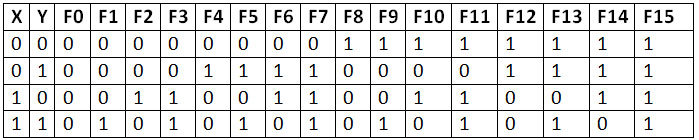
\includegraphics[scale=0.65]{twoVars.jpg}
\end{center}

Очевидно, всяка функция на $n$ променливи ще се появява и като функция на $n' > n$ променливи(т.е. $n' - n$ променливи ще са фиктивни или несъществени), при това много кратно - толкова пъти, по колкото начина можем да изберем фиктивните променливи. \par

Останалите функции от $\mathcal{F}^{2}_{2}$ зависят съществено и от двете си променливи. Ще ги означим и ще ги наричаме по следния начин:

\begin{itemize}
	\item $f_{1}(x,y) = x \wedge y = xy$ - \textit{конюнкция}. Тази функция е частен случай при $q = 2$ на функциите $min(x_{1}, x_{2})$ и $x_{1}.x_{2}(mod\;q)$;  
	\item $f_{7}(x,y) = x \vee y $ - \textit{дизюнкция}. Тази функция е частен случай при $q = 2$ на функцията $max(x_{1}, x_{2})$; 
	\item $f_{6}(x,y) = x \oplus y$ - \textit{събиране на модул 2}. Тази функция е частен случай при $q = 2$ на функцията $x_{1} + x_{2}(mod\;q)$;
	\item $f_{9}(x,y) = x \equiv y$ - \textit{еквивалентност};  
	\item $f_{13}(x,y) = x \to y$ - \textit{импликация - от $x$ следва $y$};
	\item $f_{11}(x,y) = y \to x$ - \textit{обратна импликация - от $y$ следва $x$};
	\item $f_{14}(x,y) = y | x$ - \textit{функция(черта) на Шефер};
	\item $f_{8}(x,y) = y \downarrow x$ - \textit{функция(стрелка) на Пирс};       
\end{itemize}

\subsection{Свойства}
В сила са следните:
\enumlet
\begin{enumerate}
	\item \textit{комутативни свойства:} $xy = yx, x \vee y = y \vee x, x \oplus y = y \oplus x$;
	\item \textit{асоциативни свойства:} $(xy)z = x(yz), (x \vee y) \vee z = x \vee (y \vee z), (x \oplus y)\oplus z = x \oplus (y \oplus z)$;
	\item \textit{дистрибутивни свойства:}$x(y \vee z) = xy \vee xz, x \vee yz = (x \vee y)(x \vee z), x(x \oplus z) = xy \oplus xz$;
	\item \textit{идемпотентни свойства:}$xx = x, x \vee x = x(x \oplus x) = \tilde{0}$;
	\item \textit{свойства на отрицанието:} $x\bar{x} = \tilde{0}, x \vee \bar{x} = \tilde{1}, x \oplus \bar{x} = \tilde{1}, \bar{\bar{x}} = x$;
	\item \textit{свойства на константите:} $x\tilde{0} = \tilde{0}, x\tilde{1} = x, x \vee \tilde{0} = x, x \vee \tilde{1} = \tilde{1}, x \oplus \tilde{0} = x, x \oplus \tilde{1} = \bar{x}$;
	\item \textit{закони на Де Морган:} $\overbar{x \vee y} = \bar{x} \wedge \bar{y},\overbar{x \wedge y} = \bar{x} \vee \bar{y}$;\\\\
Всяко едно от тези свойства може да се провери като директно сравним стълбовете на функциите отговарящи на двете формули. Ще използваме тези свойства, за да покажем още две:
	 \item \textit{Слепване:} Нека $f \in F_{2}$. Тогава е в сила $fx \vee f\overbar{x} = f(x \vee \overbar{x}) = f \tilde{1} = f$;
     \item \textit{Поглъщане:} Нека $f \in F_{2}$. Тогава е в сила $fg \vee f = fg \vee f\tilde{1} = f(g \vee \tilde{1} = f\tilde{1} = f$;
\end{enumerate}

\section{Формула над множество булеви функции}
\italicBold{Дефиниция:} Дефинираме индуктивно понятието формула над множество от булеви функции $F$ както следва:
\enumlet
\begin{enumerate}
	\item \textit{База:} За всяка функция $f_{i} \in F$ на $n$ променливи, думата $f_{i}(x_{1},x_{2},...x_{n} \in X^{*}$ е формула над $F$.
	\item \textit{Предположение:} Нека $f_{i} \in F$ е функция на $n$ променливи и $\phi_{1},\phi_{2},...,\phi_{n} \in X^{*}$ са формули над $F$ или променливи, т.е. от вида $x_{k}$.
	\item \textit{Стъпка:} Тогава думата $f_{i}(\phi_{1},\phi_{2},...,\phi_{n}) \in X^{*}$ е формула над $F$.
\end{enumerate}
\section{Пълни множества}
\definition С $[F]$ ще означаваме множеството от всички двоични функции, съпоставени на формулите над $F$ и ще го наричаме \textit{затваряне} на $F$ (относно суперпозицията).\\
\definition Множеството $F \subseteq \mathcal{F}_{q}$ е \textit{пълно}, ако $[F] = \mathcal{F}_{q}$.\\
Очевидно $[\mathcal{F}_{q}]=\mathcal{F}_{q}$. Но съществуването на пълни множества, различни от $\mathcal{F}_{q}$, не е очевиден факт, а е изключително важно(особено ако са с неголям брой елементи), защото позволяват да се определят класове от формули, с които се оперира много по-удобно отколкото със стълбовете на функциите.\\
Да се спрем първо на пълнотата на множества от булеви функции. \\
\definition Функцията $f(x, \sigma) = x ^{\sigma}$ дефинираме така \\
\centerline{$x^{\sigma} = 
	\begin{cases}
		x & \text{ ако } \sigma = 1 \\
		\bar{x} & \text{ ако } \sigma = 0 \\
	\end{cases}
$}\\
\lemma $x^{\sigma} = 1 \leftrightarrow x = \sigma$\\
\proof Достатъчно е да пресметнем стълба $x^{\sigma}$ и да видим, че $x^{\sigma} = x \equiv \sigma$, което доказва твърдението.
\section{Разлагане на булева функция по част от променливите}
\theorem Нека са избрани $i, 1 \leq i \leq n$ от променливите на функцията $f(x_{1}, x_{2}, ..., x_{n}) \in \mathcal{F}_{2}$ Без ограничение на общността, нека това са първите $i$ променливи. Тогава \\

\centerline{$f(x_{1}, x_{2}, ..., x_{n}) = \underset{\forall \sigma_{1}\sigma_{2}...\sigma_{i}}{\bigvee} x_{1}^{\sigma_1}x_{2}^{\sigma_2} ... x_{i}^{\sigma_i} f(\sigma_{1}, \sigma_{2}, ..., \sigma_{i}, x_{i+1}, ..., x_{n})$}
\proof Да означим с $g(x_{1}, x_{2}, ..., x_{n})$ функцията, определена от дясната част на равенството. Да пресметнем стойностите на функциите $f$ и $g$ за произволен вектор $a_{1}, a_{2}, ..., a_{n} \in J^{n}_{2}$. Вляво получаваме $f(a_{1}, a_{2}, ..., a_{n})$. От лемата, която описахме по-горе, следва че от всички $2^{i_\iota}$ елементарни конюкции $x_{1}^{\sigma_1} x_{2}^{\sigma_2} ... x_{i}^{\sigma_i}$, участващи в дясната част, само една има стойност 1 - тази, при която $\sigma_{j} = a_{j}, j = 1, 2, ..., i$. Останалите елементарни конюкции имат стойност 0 и анулират съответните членове на многократната дизюнкция. Така за стойността на дясната част получаваме:
$g(a_{1}, a_{2}, ..., a_{n}) = a_{1}^{a_1} a_{2}^{a_2} ... a_{i}^{a_i} f(a_{1}, a_{1}, ..., a_{i}, a_{i+1}, ..., a_{n})\vee \tilde{0} = \tilde{1}f(a_{1}, a_{2}, ..., a_{i}, a_{i+1},..., a_{n}) = f(a_{1}, a_{2}, ..., a_{n})$.

Следователно, функциите от двете страни на равенството съвпадат.

\section{Теорема на Бул}
\theorem Множеството $\curlies{x \vee y, xy, \bar{x}}$ е пълно\\\\
\proof Ще покажем, че $\forall \in \mathcal{F}_{2}$ е в сила $f \in [\curlies{x \vee y, xy, \bar{x}}]$, т.е. можем да представим $f$ с формула над $\curlies{x \vee y, xy, \bar{x}}$.

\enumNum
\begin{enumerate}
	\item Нека $f = \tilde{0}$. Тогава $f(x) = x\bar{x}$ и следователно $f$ се представя с форумла над $\curlies{x \vee y, xy, \bar{x}}$. 
	\item Нека $f \neq \tilde{0}$. Разлагаме $f(x_{1}, x_{2}, ..., x_{n})$ по всичките $n$ променливи и получаваме \\
		\centerline{$f(x_{1}, x_{2}, ..., x_{n}) = \underset{\forall \sigma_{1}\sigma_{2}...\sigma_{n}}{\bigvee}x_{1}^{\sigma_1} x_{2}^{\sigma_2} ... x_{n}^{\sigma_n} f(\sigma_{1}, \sigma_{2}, ..., \sigma_{n})$.}
\end{enumerate}

Ако $f(\sigma_{1}, \sigma_{2}, ..., \sigma_{n}) = 0$, съответният член в дясната част се анулира и съгласно свойствата, доказани по-горе, може да не участва във формулата. Ако пък $f(\sigma_{1}, \sigma_{2}, ..., \sigma_{n}) = 1$, то $x_{1}^{\sigma_1}x_{2}^{\sigma_2}... x_{n}^{\sigma_n} f(\sigma_{1}, \sigma_{2}, ..., \sigma_{n}) = x_{1}^{\sigma_1}x_{2}^{\sigma_2}... x_{n}^{\sigma_n}$. Така получаваме $f(x_{1}, x_{2}, ..., x_{n}) =   \bigvee_{\substack{\forall \sigma_{1} \sigma{2}...\sigma{n} \\ f(\sigma_{1} \sigma{2}...\sigma{n}) = 1}} x_{1}^{\sigma_1}x_{2}^{\sigma_2}...x_{n}^{\sigma_n}$, което е формула над $\curlies{x \vee y, xy, \bar{x}}$.

\section{Теорема на Пост-Яблонски}
\theorem Нека $F \subseteq \mathcal{F}^{n}_{2}$. Множеството $F$ е пълно $\leftrightarrow$, когато \\
\centerline{$F\not\subseteq T_{0}\;\&\;F \not\subseteq T_{1}\;\&\;F \not\subseteq S\;\&\;F \not\subseteq M\;\&\;F \not\subseteq L$}
\end{document}
